\documentclass[0-protokol.tex]{subfiles}
\begin{document}

\subsection*{Metoda přímá}
Přímá metoda měření odporu spočívá v měření napětí a proudu, protékajícího odporem, pomocí zapojení 1 $a$ či $b$. Problém této metody je, že při zapojení $a$ měříme kromě napětí na odporu i napětí ampérmetru. Naopak zapojením $b$ měříme proud, protékající odporem i voltmetrem. 

Výsledný odpor bez korekce spočítáme podle známého vztahu
\begin{equation}
R = \frac{U}{I},
\end{equation}
kde $U$ a $I$ jsou naměřené hodnoty napětí a proudu. Chceme-li provézt korekci na uvedené nedostatky této metody, použijeme pro $a$ vzorec
\begin{equation}
R = \frac{U}{I}  - R_A,
\end{equation}
kde $R_A$ je odpor ampérmetru, pro $b$ vzorec
\begin{equation}
R = \frac{R_V U}{R_V I - U},
\end{equation}
kde $R_V$ je odpor voltmetru.

\begin{figure}[H] \label{fig:zap1_2}
\centering
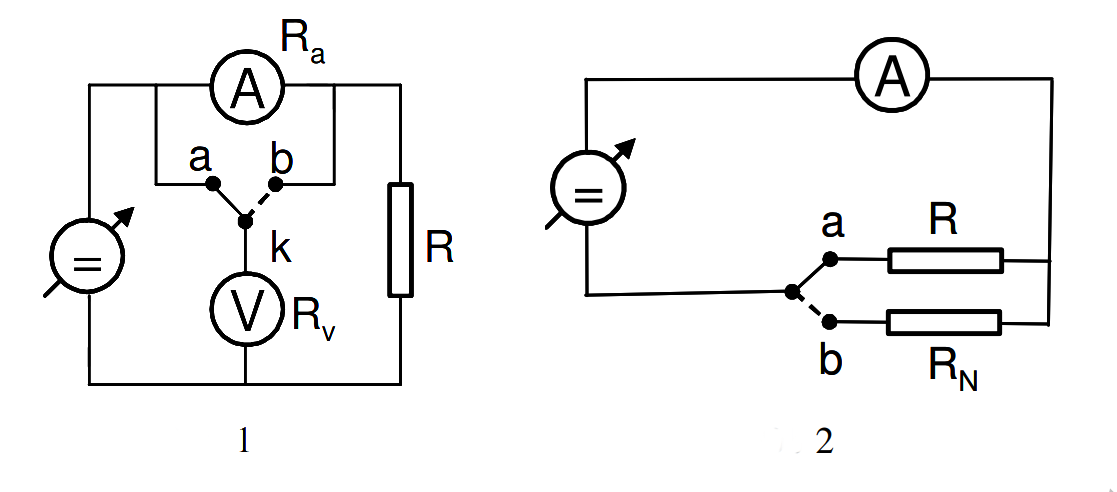
\includegraphics[scale=0.4]{plot/zap1_2}
\caption{Použitá zapojení \cite{stud_text}}
\end{figure}

\subsection*{Metoda substituční}
Tato metoda měření odporu je přesnější než metoda přímá, protože při měření podle zapojení 2 srovnáváme měřený odpor se známou hodnotou odporu na odporové dekádě za konstantního proudu. Nevzniká při tom takové zkreslení naměřené hodnoty. Nejprve při zapojení $a$ nastavíme určitou hodnotu proudu na ampérmetru. Následně přepneme na zapojení $b$ a měněním odporu na odporové dekádě uvedeme hodnotu proudu na ampérmetru na totožnou hodnotu. Nakonec odečteme výsledný odpor z odporové dekády.

\subsection*{Extrapolace odporu žárovky při pokojové teplotě}
Při malém odporu se většina energie přemění v Joulovo teplo, pro příkon pak platí
\begin{equation}
P = U I = k \Delta T,
\end{equation}
kde $k$ je konstanta úměrnosti a $\Delta T$ je rozdíl mezi teplotou vlákna a pokojovou teplotou. Pro malé rozsahy teplot kolem pokojové teploty uvažujeme
\begin{equation}
R = R_0 (1 + \alpha \Delta T),
\end{equation}
přičemž $R_0$ je odpor vlákna při pokojové teplotě. 

Z těchto vzorců dostaneme
\begin{equation}
R = R_0 + \frac{R_0 \alpha}{k}P,
\end{equation}
tedy odpor je přímo úměrný příkonu. Lineární regresi můžeme provézt pro
\begin{equation} \label{eq:regrese}
R = R_0 + K P,
\end{equation}
kde $K = \frac{R_0 \alpha}{k}$.

\end{document}
